\section{Association plots}\label{sec:twoway-assoc}
In the \IX{sieve diagram} the foreground (rectangles) shows expected
frequencies; deviations from independence are shown by color and
density of shading.  The association plot
\citep{Cohen:80,Friendly:91}
puts deviations from independence in the foreground:  the area
of each box is made proportional to observed $-$ expected frequency.
This graphical method is described in more detail in \SSSGref{10.2.1},
which also lists the program used to produce the association plot.

For a two-way contingency table, the signed contribution to Pearson
\(\chi^2\) for cell \(i, \, j\) is
\begin{equation*}
  d_{ij}  =
  \frac{ n_{ij} - m_{ij} } { \sqrt { m_{ij} } }
 = \mbox{ std. residual},
  \qquad
  \chi^2 = \sum_{ij} \:  ( d_{ij} )^2
\end{equation*}

In the \glossterm{association plot}, each cell is shown by a
rectangle:

\begin{itemize*}
\item (signed) height \(\sim d_{ij}\)

\item width = \(\sqrt { m_{ij}}\).
\end{itemize*}
so, the area of each cell is proportional to the raw residual,
\glosstex{residuals}
\(n_{ij} - m_{ij}\).
The rectangles for each row in the table are positioned relative to a
baseline representing independence (\(d_{ij} = 0\)) shown by a dotted
line.  Cells with observed \(>\) expected frequency rise above the line
(and are colored black); cells that contain less than the expected
frequency fall below it (and are shaded gray).

\begin{figure}[htb]
  \centering
  \includegraphics[width=.7\linewidth]{ch3/fig/assocplt.eps}
  \caption{Association plot for hair-color, eye-color.}\label{fig:assocplt}
\end{figure}
\figref{fig:assocplt} shows the association plot for the hair-color,
eye-color data.  Note that the residuals in each row tend to increase
or decrease systematically in each row, except that for hazel eyes.

One virtue of the association plot is that it is quite simple to
interpret.  
\citet{Bertin:81} uses similar graphics to display large complex
\ctabs.  Like the sieve diagram, however, patterns of association
are most apparent when the rows and columns of the display are ordered
in a sensible way.
